\section{Programmentwurf \textnormal{\textsf{\small{Christian Sasse}}}}

\subsection{Use-Case-Diagramm}
In Use-Case-Diagrammen wird das externe Systemverhalten aus Anwendersicht beschrieben. Sie stellen das geplante System, die Akteure, die Verwendung des geplanten Systems (Anwendungsfälle) und die Beziehungen zwi­schen Akteuren und Anwendungsfällen dar. Kurz gesagt: Use Case Diagramme geben Auskunft darüber, was ein geplantes System aus Sichtweise der Benutzer leisten soll. In dem in dieser Arbeit behandelten Planspiel soll das Use Case Diagramm zeigen, was der Akteur, also der Spieler, alles steuern kann.
Das Use-Case Diagramm besteht aus folgenden Elementen:

\begin{description}
\item[Use Case (Anwendungsfall)]
 Ein Anwendungsfall ist ein in sich abgeschlossener Vorgang, der für einen oder mehrere Akteure ein beobachtbares Ergebnis liefert. Er beschreibt aus Sicht der Akteure welche Leistungen das System für den Anwender zur Verfügung stellt. Ein Use Case stellt somit einen Teil der Gesamtfunktionalität des Systems dar. es wird durch eine Ellipse dargestellt. 

\item[Akteur]
Der Akteur ist ein Element, das nicht zum geplanten System gehört. Er kann eine Person sein, die auf das System zugreift, oder ein anderes System, das mit dem geplanten System kommuniziert. In diesem Planspiel ist der Akteur somit der Spieler und wird als Strichmännchen dargestellt.

\item[Assoziation]
Eine Linie stellt eine Assoziation zwischen einem Akteur und einem Use Case dar. Sie beschreibt den Zugriff des Akteurs auf die Funktionalität, die das System in diesem Use Case zur Verfü­gung stellt, bzw. eine Antwort des Systems an einen Akteur. In Abbildung \ref{abb:use_case_assoziation} wird eine solche Assoziation dargestellt. dort ist zu sehen, dass der Akteur einen Mitarbeiter einstellen kann.
\begin{figure}[h]
	\centering	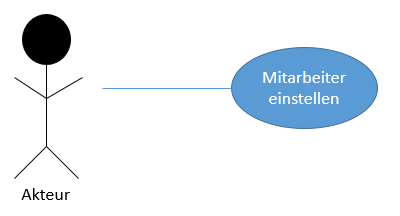
\includegraphics[width=0.5\textwidth]{img/programmentwurf/use_case_assoziation}
	\captionsetup{format=hang}
	\caption{
		\label{abb:use_case_assoziation}Assoziation in einem Use-Case-Diagramm}
\end{figure}

\item[Include-Assoziation]
Bei der Include-Beziehung verwendet ein Use Case die Funktionalität, die ein anderer Use Case zur Verfügung stellt. Der inkludierte Use Case wird immer ausgeführt. Dies ist in Abbildung \ref{abb:use_case_include} zu sehen. Hier ist zu erkennen, dass der von dem Akteur eingestellte Mitarbeiter einer Abteilung zugewiesen wird.



\begin{figure}[h]
	\centering	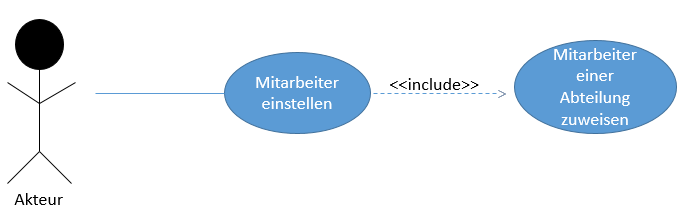
\includegraphics[width=0.5\textwidth]{img/programmentwurf/use_case_include}
	\captionsetup{format=hang}
	\caption{
		\label{abb:use_case_include}Include-Assoziation}
\end{figure}

\item[Extend-Assoziation]
Die Extend Beziehung, beschreibt die Erweiterung der Funktionalität eines Use Cases durch einen anderen Use Case. Man kann dadurch optionales Verhalten beschreiben, bzw. Funktionen modellieren, die nur unter bestimmten Bedingungen ausgeführt werden. Die folgende Abbildung zeigt eine solche Beziehung, wie sie im Planspiel auftritt. Der Akteur hat die Wahl, den Bestand der zu produzierenden Produkte zu verändern.
\begin{figure}[h]
	\centering	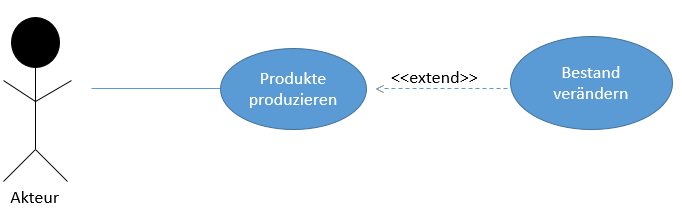
\includegraphics[width=0.5\textwidth]{img/programmentwurf/use_case_extend}
	\captionsetup{format=hang}
	\caption{
		\label{abb:use_case_extend}Extend-Assoziation}
\end{figure}

\end{description}

Neben den oben genannten Use Cases, soll es dem Spieler, wie in Abbildung \ref{abb:usecase} zu sehen, weiterhin möglich sein Produkte zu erforschen. Nach Abschluss eines Forschungsprojektes stehen verbesserte Produkte zur Verfügung.
Ein weiterer Anwendungsfall soll das Durchführen einer Markforschung sein. Hierdurch können zum Beispiel Zielgruppen besser angesprochen werden, wodurch sich Produkte besser verkaufen lassen.

 
\begin{figure}[h]
	\centering	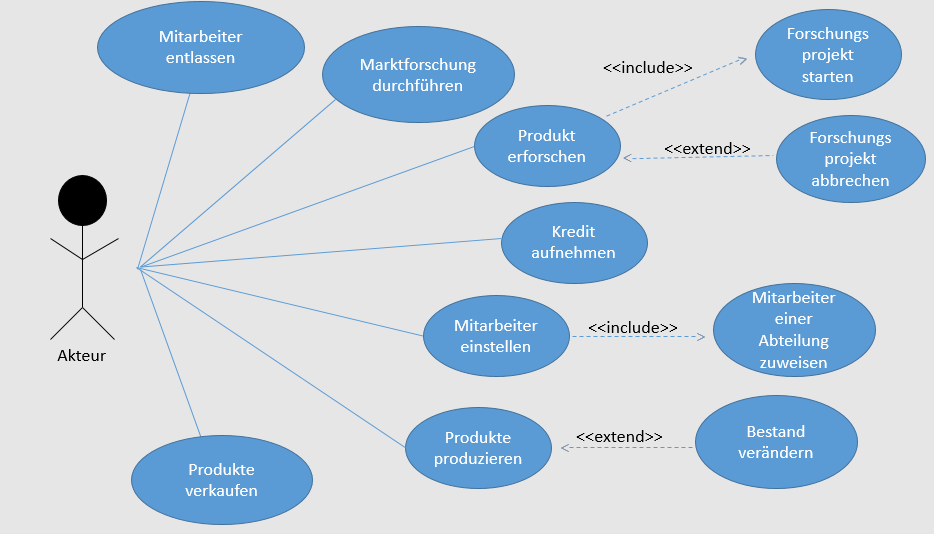
\includegraphics[width=0.5\textwidth]{img/programmentwurf/usecase}
	\captionsetup{format=hang}
	\caption{
		\label{abb:usecase}Use Case Diagramm}
\end{figure}


\subsection{Klassendiagramm}

Um die Zusammenhänge zwischen den Klassen sowie deren Aufbau zu veranschaulichen, wird ein Klassendiagramm verwendet.
Ein Klassendiagramm ist ein Strukturdiagramm der Unified Modeling Language (UML) zur grafischen Darstellung (Modellierung) von Klassen, Schnittstellen sowie deren Beziehungen.

Als \enquote{Kopf} des Planspiels dient die Klasse \texttt{Game}. Hier werden die verschiedenen Unternehmen der Spieler gelistet und die Spielzeit gesetzt und verwaltet. 

\begin{figure}[h]
	\centering	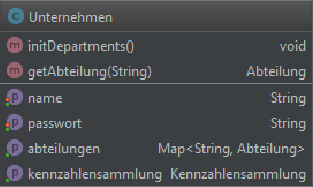
\includegraphics[width=0.5\textwidth]{img/programmentwurf/unternehmen_klasse}
	\captionsetup{format=hang}
	\caption{
		\label{abb:unternehmen_klasse}Aufbau der Klasse \enquote{Unternehmen}}
\end{figure}

In Abbildung \ref{abb:unternehmen_klasse} ist der typische Aufbau einer Klasse in UML zu sehen. Diese werden in die drei Rubriken - Klassenname, Attribute, Operationen - jeweils durch eine horizontale Linie aufgeteilt.

Die Attribute einer Klasse werden mit ihrem Namen aufgeführt und enthalten zusätzlich Angaben zu ihren Eigenschaftswerten. Methoden werden ebenfalls mit ihrem Namen, zusätzlich mit möglichen Parametern und dem Rückgabewert notiert. 

Betrachtet man die oben abgebildete \texttt{Unternehmen}-Klasse, sieht man dass dort der Name und das Passwort eines Unternehmens gesetzt werden und dessen Abteilungen und Kennzahlensammlung als Attribute enthalten sind.
Die Methode \texttt{initDepartments()} dient zum Initialiseren der Abteilungen.

Die Beziehungen zwischen den Klassen werden durch vier verschiedene Arten verdeutlicht:

\begin{description}
	\item[Assoziation]
	Beschreibt eine Beziehung zwischen zwei oder mehr Klassen. An den Enden von Assoziationen sind häufig Multiplizitäten vermerkt. Diese drücken aus, wie viele dieser Objekte in Relation zu den anderen Objekten dieser Assoziation stehen.
	\item[Aggregation (Teil-eines-Ganzen-Beziehung)]
	Liegt dann vor, wenn zwischen den Objekten der beteiligten Klassen eine Beziehung besteht,	die sich als \enquote{ist Teil von} oder \enquote{besteht aus} beschreiben lässt, also ein Objekt aus Teil-Objekten besteht.
	\item[Komposition]
	Ist eine starke Form der Aggregation und bildet den Fall ab, bei dem die Teile nicht ohne das Ganze existieren können. 
	
	Abbildung \ref{abb:unternehmen_abteilung_beziehung} stellt eine solche Beziehung dar. Die in Abbildung \ref{abb:unternehmen_klasse} gezeigte \texttt{Unternehmen}-Klasse erhält nun eine Teilklasse namens \enquote{Abteilung}, welche ohne das Unternhemen nicht existieren kann.
		\begin{figure}[h]
		\centering	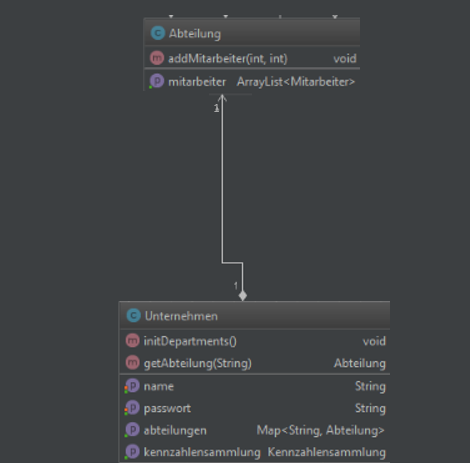
\includegraphics[width=0.5\textwidth]{img/programmentwurf/unternehmen_abteilung_beziehung}
	\captionsetup{format=hang}
	\caption{
		\label{abb:unternehmen_abteilung_beziehung}Beziehung der Klassen \enquote{Unternehmen} und \enquote{Abteilung}}
	\end{figure}

	Somit herrscht auch zwischen der \texttt{Game}-Klasse und der \texttt{Unternehmen}-Klasse eine Komposition, da es ohne das Game kein Unternehmen geben würde.
	
	\item[Create-Abhängigkeit]
	Hier erzeugt ein abhängiges Element Exemplare des unabhängigen Elementes. 
	Dargestellt wird eine dies durch einen mit \texttt{<<create>>} beschrifteten, gestrichelten Pfeil, wobei der Pfeil vom abhängigen auf das unabhängige Element zeigt.
	Durch die oben erwähnte \texttt{initDepartments()}-Methode der \texttt{Unternehmen}-Klasse, geht diese eine solche Abhängigkeit mit den gesamten Abteilungen des Unternehmens ein.
		
	\item[Generalisierung (Ist-ein-Beziehung)]
	Liegt dann vor, wenn zwischen den Objekten der beteiligten Klassen eine Beziehung besteht, die sich als \enquote{ist ein} beschreiben lässt. Das heißt, es existiert eine generellere und eine speziellere Klasse. Exemplare der spezielleren Klasse sind damit auch Exemplare der generelleren Klasse. Konkret bedeutet dies, dass die speziellere Klasse über alle Merkmale (Struktur- und Verhaltensmerkmale) der generelleren Klasse verfügt.

	Die folgende Abbildung \ref{abb:abteilungen} zeigt die Abteilungsklasse, welche als generelle Klasse dient, mit ihren spezielleren Klassen, den einzelnen Abteilungen des Unternehmens.
	\begin{figure}[h]
		\centering	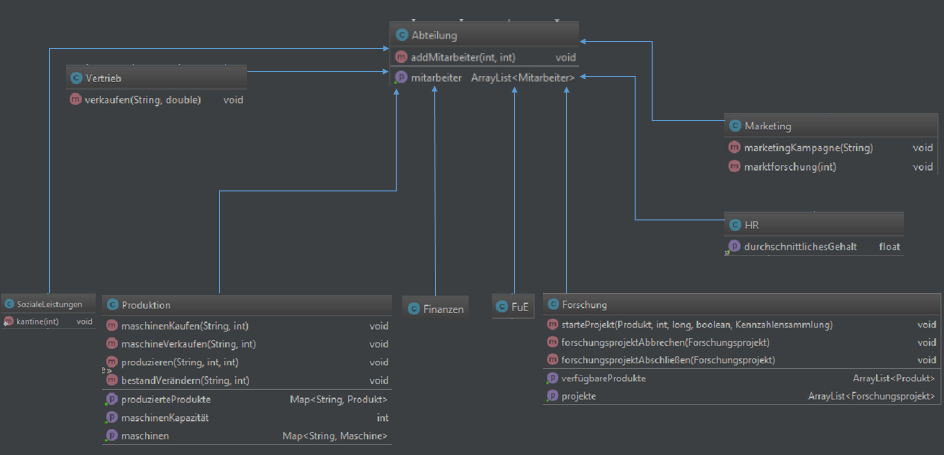
\includegraphics[width=0.57\textwidth]{img/programmentwurf/abteilungen}
		\captionsetup{format=hang}
		\caption{
			\label{abb:abteilungen}Abteilungen der Klasse \enquote{Abteilung}}
	\end{figure}	
\end{description}

Die eben gezeigte Generalisierung findet deshalb Anwendung, weil es für die Mitarbeiter der einzelnen Abteilungen noch eine eigene Klasse gibt, die eine Komposition mit der \texttt{Abteilung}-Klasse eingeht. Über deren Methode \texttt{addMitarbeiter()} können den einzelnen Abteilungen dann Mitarbeiter hinzugefügt werden. Jede Abteilung kann dabei beliebig viele Mitarbeiter enthalten. Umgekehrt kann ein Mitarbeiter jedoch immer nur in einer Abteilung arbeiten.


Die Kennzahlen eines Unternehmens, wie Fremdkapital, Eigenkapital oder Bekanntheitsgrad werden in der
\texttt{Kennzahlensammlung}-Klasse verwaltet. Jede Kennzahl erhält hierbei ihre eigene Klasse. Da die ganzen Kennzahlen jedoch gleiche Methoden, wie z.B. \texttt{berechnen()} und gleiche Eigenschaften, wie z.B. \texttt{wert} besitzen, ist es hier auch sinnvoll eine generelle Klasse zu erstellen, die diese gleichen Methoden und Eigenschaften besitzt. Diese Klasse trägt den Namen \texttt{Kennzahl}. Zu sehen ist diese Verbindung in Abbildung \ref{abb:kennzahlen_verbindung}. Innerhalb der \texttt{Kennzahlensammlung}-Klasse werden die einzelnen Kennzahlen berechnet. In der \texttt{Unternhemen}-Klasse können diese dann abgefragt werden.
	\begin{figure}[h]
	\centering	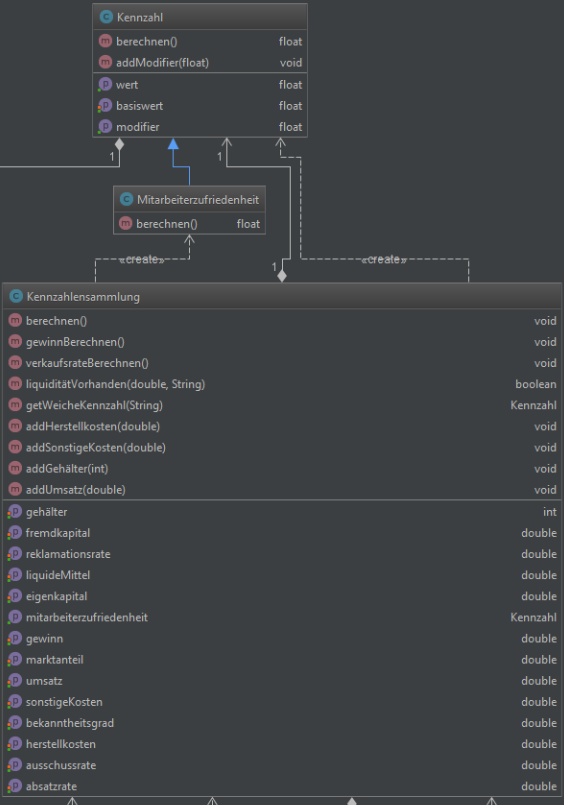
\includegraphics[width=0.5\textwidth]{img/programmentwurf/kennzahlen_verbindung}
	\captionsetup{format=hang}
	\caption{
		\label{abb:kennzahlen_verbindung}Abteilungen der Klasse \enquote{Abteilung}}
\end{figure}	

Mithilfe der Klasse \texttt{Produktion} können Produkte produziert werden. Für die Produktion werden jedoch Maschinen benötigt, die auch innerhalb der Klasse gekauft werden können. Für die Maschinen selbst gibt es wiederum eine eigene Klasse, die deren Kapazität, Klasse, Anzahl und Anschaffungskosten als Attribute enthält.
Auch für die Produkte gibt es eine eigene Klasse. Sie enthält neben dem Namen und der Anzahl auch den Preis und die Herstellungskosten als Attribute. Die \texttt{Produkt}-Klasse ist ein Teil der Produktion und könnte ohne diese nicht existieren, also herrscht hier eine Komposition. Des weiteren kann eine Produktion nur ein Produkt beinhalten. 
Produzierte Produkte können innerhalb der Klasse \texttt{Vertrieb} verkauft werden.

Die Produktforschung findet innerhalb der Klassen \texttt{Forschung} und \texttt{Forschungsprojekt} statt. 
Die Klasse \texttt{Forschung} kann hierbei beliebig viele Forschungsprojekte, gelistet im Attribut \texttt{projekte}, enthalten. Die Beziehung zwischen den beiden Klassen ist eine Komposition, da ein Forschungsprojekt ohne die Abteilung Forschung nicht existieren kann. Weiterhin kann in einem Forschungsprojekt nur ein Produkt erforscht werden. Diese Beziehung ist eine Aggregation. Ein Forschungsprojekt enthält als Eigenschaften die Dauer, das zu erforschende Produkt, den Beginn der Forschung und die Anzahl der Mitarbeiter. Man kann es starten, abbrechen und abschließen.

Die folgende Abbildung \ref{abb:klassendiagramm} zeigt das komplette Klassendiagramm. Dort sind die oben beschriebenen Beziehungen zwischen den einzelnen Klassen zu erkennen. Zu erwähnen ist, dass das Klassendiagramm nur als Grundkonzept innerhalb der Entwurfsphase dient und nicht alle Funktionen der Endanwendung widerspiegelt. Deshalb sind einige Klassen noch nicht ausgearbeitet und haben keine erkennbare Funktion. Weiterhin sind dort noch nicht alle Klassen der Kennzahlen vorhanden und es noch keine Möglichkeit seine Finanzen oder Aufträge zu verwalten.

\begin{figure}[h]
	\centering	\includegraphics[width=\textwidth]{img/programmentwurf/klassendiagramm}
	\captionsetup{format=hang}
	\caption{
		\label{abb:klassendiagramm}Vollständiges Klassendiagramm}
\end{figure}




